\documentclass[11pt]{article}
\usepackage[margin=1in]{geometry}
\usepackage{booktabs}
\usepackage{amsmath}
\usepackage{amssymb}
\usepackage{graphicx}
\usepackage{xcolor}
\usepackage{caption}
\usepackage{capt-of}
\usepackage{tikz}
\usetikzlibrary{arrows.meta}
\title{LoCoBench: Logical Coherence Score Evaluation\\
\large The gold-relation arm on generated items}
\author{FactReasoner --- LoCoBench evaluation}
\date{\today}


\begin{document}

\maketitle

\section{Setup}

This report evaluates the Logical Coherence Score (LCS) pipeline on the \textbf{10 generated items} of \texttt{locobench-claude-5}. Unlike the mining experiments, relations are \emph{not} mined by a model here: each item already carries its inter-atom relations as gold labels, and those labels are compiled directly into the coherence MRF. No LLM is involved, so every number below is deterministic and reproducible offline (Merlin is the only subprocess).

\paragraph{Atom priors.} An atom's unary factor is $[1-\pi_i, \pi_i]$ with $\pi_i = 0.9$ when the item marks the atom \texttt{factual} and $\pi_i = 0.1$ when it does not. The coherence MRF therefore starts from the corpus's own factuality labels --- the label-driven analogue of the two-stage model, where stage~1's posterior marginals play this role. Hard $1/0$ priors are deliberately avoided: they would zero out worlds and make several readouts degenerate.

\paragraph{Edge probabilities.} A gold relation carries an intended strength band and a strength range; the factor probability is the range's \textbf{midpoint} (strong $[0.85,1] \to 0.925$, moderate $[0.6,0.84] \to 0.720$, weak $[0.35,0.59] \to 0.470$). Because gold is a \emph{label} rather than an estimate, the type confidence $P(\tau \mid a_i,a_j)$ is fixed at $1.0$ and the conditional strength is that same midpoint. Any apparent precision beyond the band is an artefact of the midpoint convention, not a measurement.

\paragraph{Resolved concessions.} A concession the text resolves is softened by $p \mapsto p\,(1-\lambda)$ with $\lambda = 0.45$ (deep-dive Eq.~2). The resolver is read from the item's own \texttt{resolver\_atom\_id}, so the miner's text heuristic for spotting a holding atom is bypassed entirely --- when the label states the resolver, guessing it would be the wrong instrument.

\paragraph{Ordering-only relations.} \texttt{Precedence} and \texttt{Succession} compile to Level-1 \texttt{none}: they record source/target order but couple no truth values, so they contribute \textbf{no factor}. They are counted in the dataset table and excluded from the MRF, exactly as \texttt{lcs.taxonomy.compile\_sense} dictates.

\paragraph{Arms.} Each item is scored under \textbf{\texttt{gold}} (all gold edges) and \textbf{\texttt{gold\_valid}} (valid edges only). The second arm drops the deliberately-planted invalid relations, which isolates what those planted errors cost. All four readouts are computed for both: \texttt{mean\_marginal}, \texttt{consistency}, \texttt{reified}, \texttt{log\_partition}.

\section{Dataset}

\begin{table}[htbp]
\centering
\small
\caption{Per-item size. \textbf{Gold} is every relation the item lists; \textbf{ord-only} are the Precedence/Succession edges that carry no truth coupling and so produce no factor; \textbf{MRF} is what remains and is scored; \textbf{valid} is the subset whose \texttt{validity} is \texttt{valid}.}
\label{tab:dataset}
\begin{tabular}{lllrrrrr}
\toprule
Family & Rung & Name & Atoms & Gold & ord-only & MRF & valid \\
\midrule
\texttt{f001} & 0 & worse & 16 & 10 & 1 & 9 & 5 \\
\texttt{f001} & 1 & base & 16 & 10 & 1 & 9 & 5 \\
\texttt{f001} & 2 & concession\_resolved & 16 & 10 & 1 & 9 & 5 \\
\texttt{f001} & 3 & fix\_one\_conflict & 16 & 10 & 1 & 9 & 5 \\
\texttt{f001} & 4 & coherent & 16 & 10 & 1 & 9 & 5 \\
\texttt{f002} & 0 & worse & 16 & 10 & 1 & 9 & 5 \\
\texttt{f002} & 1 & base & 16 & 10 & 1 & 9 & 5 \\
\texttt{f002} & 2 & concession\_resolved & 16 & 10 & 1 & 9 & 5 \\
\texttt{f002} & 3 & fix\_one\_conflict & 16 & 10 & 1 & 9 & 5 \\
\texttt{f002} & 4 & coherent & 16 & 10 & 1 & 9 & 5 \\
\bottomrule
\end{tabular}
\end{table}

Across the dataset there are 160 atoms, of which 140 are marked \texttt{factual} (prior 0.9) and 20 are not (prior 0.1).

\begin{minipage}[t]{0.48\linewidth}
\centering
\small
\captionof{table}{Level-2 discourse senses.}
\label{tab:senses}
\begin{tabular}{lr}
\toprule
Value & Count \\
\midrule
\texttt{Alternative} & 15 \\
\texttt{Concession} & 15 \\
\texttt{Contrast} & 15 \\
\texttt{Disjunction} & 10 \\
\texttt{Evidence} & 10 \\
\texttt{Instantiation} & 10 \\
\texttt{Precedence} & 10 \\
\texttt{Restatement} & 10 \\
\texttt{Cause-Effect} & 5 \\
\bottomrule
\end{tabular}
\end{minipage}\hfill\begin{minipage}[t]{0.48\linewidth}
\centering
\small
\captionof{table}{Level-1 couplings.}
\label{tab:couplings}
\begin{tabular}{lr}
\toprule
Value & Count \\
\midrule
\texttt{contradiction} & 30 \\
\texttt{entailment} & 25 \\
\texttt{exclusive} & 15 \\
\texttt{co\_necessity} & 10 \\
\texttt{equivalence} & 10 \\
\texttt{none} & 10 \\
\bottomrule
\end{tabular}
\end{minipage}

\bigskip
\begin{minipage}[t]{0.48\linewidth}
\centering
\small
\captionof{table}{Relation validity.}
\label{tab:validity}
\begin{tabular}{lr}
\toprule
Value & Count \\
\midrule
\texttt{valid} & 60 \\
\texttt{invalid} & 40 \\
\bottomrule
\end{tabular}
\end{minipage}\hfill\begin{minipage}[t]{0.48\linewidth}
\centering
\small
\captionof{table}{Planted error kinds.}
\label{tab:errorkinds}
\begin{tabular}{lr}
\toprule
Value & Count \\
\midrule
\texttt{false\_endpoint} & 20 \\
\texttt{wrong\_direction} & 10 \\
\texttt{wrong\_sense} & 10 \\
\bottomrule
\end{tabular}
\end{minipage}

\noindent 40 of 100 gold relations (40\%) are deliberately invalid: the corpus plants relation-level errors so a system's ability to \emph{recover} the intended graph can be graded. The \texttt{gold} arm scores the graph as labelled, including those errors; the \texttt{gold\_valid} arm scores only the intended-correct subgraph.

\section{LCS scores}

\begin{table}[htbp]
\centering
\small
\caption{LCS readouts, arm \texttt{gold} (all gold edges). Higher is more coherent for every readout. \textbf{Rel} is the number of edge-producing relations in the MRF.}
\label{tab:scores-gold}
\begin{tabular}{llrrrrrr}
\toprule
Family & Rung & Rel & \textbf{mean-marg} & \textbf{consist} & \textbf{reified} & \textbf{log-Z} & $\log Z$ \\
\midrule
\texttt{f001} & 0 (worse) & 9 & 0.799 & 0.029 & 0.208 & 0.315 & -5.11 \\
\texttt{f001} & 1 (base) & 9 & 0.799 & 0.029 & 0.208 & 0.315 & -5.11 \\
\texttt{f001} & 2 (concession\_resolved) & 9 & 0.799 & 0.029 & 0.208 & 0.315 & -5.11 \\
\texttt{f001} & 3 (fix\_one\_conflict) & 9 & 0.799 & 0.029 & 0.208 & 0.315 & -5.11 \\
\texttt{f001} & 4 (coherent) & 9 & 0.799 & 0.029 & 0.208 & 0.315 & -5.11 \\
\midrule
\texttt{f002} & 0 (worse) & 9 & 0.792 & 0.304 & 0.330 & 0.367 & -5.25 \\
\texttt{f002} & 1 (base) & 9 & 0.792 & 0.304 & 0.330 & 0.367 & -5.25 \\
\texttt{f002} & 2 (concession\_resolved) & 9 & 0.792 & 0.304 & 0.330 & 0.367 & -5.25 \\
\texttt{f002} & 3 (fix\_one\_conflict) & 9 & 0.792 & 0.304 & 0.330 & 0.367 & -5.25 \\
\texttt{f002} & 4 (coherent) & 9 & 0.792 & 0.304 & 0.330 & 0.367 & -5.25 \\
\bottomrule
\end{tabular}
\end{table}

\begin{table}[htbp]
\centering
\small
\caption{LCS readouts, arm \texttt{gold\_valid} (valid edges only). Higher is more coherent for every readout. \textbf{Rel} is the number of edge-producing relations in the MRF.}
\label{tab:scores-gold-valid}
\begin{tabular}{llrrrrrr}
\toprule
Family & Rung & Rel & \textbf{mean-marg} & \textbf{consist} & \textbf{reified} & \textbf{log-Z} & $\log Z$ \\
\midrule
\texttt{f001} & 0 (worse) & 5 & 0.790 & 0.320 & 0.353 & 0.480 & -2.99 \\
\texttt{f001} & 1 (base) & 5 & 0.790 & 0.320 & 0.353 & 0.480 & -2.99 \\
\texttt{f001} & 2 (concession\_resolved) & 5 & 0.790 & 0.320 & 0.353 & 0.480 & -2.99 \\
\texttt{f001} & 3 (fix\_one\_conflict) & 5 & 0.790 & 0.320 & 0.353 & 0.480 & -2.99 \\
\texttt{f001} & 4 (coherent) & 5 & 0.790 & 0.320 & 0.353 & 0.480 & -2.99 \\
\midrule
\texttt{f002} & 0 (worse) & 5 & 0.790 & 0.349 & 0.362 & 0.494 & -2.93 \\
\texttt{f002} & 1 (base) & 5 & 0.790 & 0.349 & 0.362 & 0.494 & -2.93 \\
\texttt{f002} & 2 (concession\_resolved) & 5 & 0.790 & 0.349 & 0.362 & 0.494 & -2.93 \\
\texttt{f002} & 3 (fix\_one\_conflict) & 5 & 0.790 & 0.349 & 0.362 & 0.494 & -2.93 \\
\texttt{f002} & 4 (coherent) & 5 & 0.790 & 0.349 & 0.362 & 0.494 & -2.93 \\
\bottomrule
\end{tabular}
\end{table}

\subsection{Effect of the planted invalid relations}

Removing the deliberately-invalid gold relations is the clearest single-number effect in this evaluation. The planted errors are predominantly conflict edges attached to a false endpoint, so deleting them removes active contradictions: the conflict-sensitive readouts move sharply, while \texttt{mean\_marginal} --- an average over atom marginals already pinned near their $0.9/0.1$ priors --- barely moves.

\begin{table}[htbp]
\centering
\small
\caption{Change in each readout from arm \texttt{gold} to arm \texttt{gold\_valid} (valid edges only). Positive means the intended-correct subgraph scores as more coherent.}
\label{tab:arm-delta}
\begin{tabular}{llrrrrr}
\toprule
Family & Rung & Rel & \textbf{mean-marg} & \textbf{consist} & \textbf{reified} & \textbf{log-Z} \\
\midrule
\texttt{f001} & 0 & 9 $\to$ 5 & -0.009 & +0.291 & +0.145 & +0.165 \\
\texttt{f001} & 1 & 9 $\to$ 5 & -0.009 & +0.291 & +0.145 & +0.165 \\
\texttt{f001} & 2 & 9 $\to$ 5 & -0.009 & +0.291 & +0.145 & +0.165 \\
\texttt{f001} & 3 & 9 $\to$ 5 & -0.009 & +0.291 & +0.145 & +0.165 \\
\texttt{f001} & 4 & 9 $\to$ 5 & -0.009 & +0.291 & +0.145 & +0.165 \\
\texttt{f002} & 0 & 9 $\to$ 5 & -0.003 & +0.046 & +0.032 & +0.127 \\
\texttt{f002} & 1 & 9 $\to$ 5 & -0.003 & +0.046 & +0.032 & +0.127 \\
\texttt{f002} & 2 & 9 $\to$ 5 & -0.003 & +0.046 & +0.032 & +0.127 \\
\texttt{f002} & 3 & 9 $\to$ 5 & -0.003 & +0.046 & +0.032 & +0.127 \\
\texttt{f002} & 4 & 9 $\to$ 5 & -0.003 & +0.046 & +0.032 & +0.127 \\
\bottomrule
\end{tabular}
\end{table}

\section{Ladder ordering constraints}\label{sec:ladder}

Each family declares the ordering its rungs are meant to exhibit; the graded readouts are \texttt{mean\_marginal}, \texttt{consistency}, \texttt{log\_partition}.

\paragraph{The gold relations do not vary across a family's rungs.} In \texttt{f001}, \texttt{f002}, every rung carries a byte-identical gold relation set while the response \emph{texts} differ per rung. The generator perturbs each rung's prose but re-attaches the base plan's relation list to all five items, so the labels describe the base ladder rather than the rung they ship with. \textbf{Consequence:} the gold-relation MRF is identical across a family's rungs, the scores below are constant within a family, and the ordering constraints --- which assert a \emph{strict increase} in coherence up the ladder --- cannot be satisfied by construction. The pass/fail tables that follow therefore measure the corpus, not the LCS pipeline. Testing the ladder itself requires per-rung relations, either by fixing the generator or by mining each rung's own text.

\paragraph{The generator has since been fixed.} The defect is closed in \texttt{locobench.pipeline}: a rung's gold relations are now the base edge set with that rung's own perturbations applied (\texttt{perturb.apply\_calls}), each call targets a distinct eligible edge (\texttt{perturb.plan\_targets} --- previously every call was passed the hardcoded edge \texttt{r000}), and a rung whose edge set still matches its parent's while its calls claim a change is now rejected outright. Applying those transforms to this dataset's base rungs makes $\log Z$ strictly monotone up both ladders, where it is flat here. \textbf{The tables in this report describe the dataset as it exists on disk}, generated before that fix; regenerating it requires new model calls and has not been done.

\subsection*{Family \texttt{f001} (Anthropology, CONFLICT)}

Gold relations identical across rungs: \textbf{yes}; distinct response texts: 5 of 5.

\begin{table}[htbp]
\centering
\small
\caption{Ordering constraints for \texttt{f001}, arm \texttt{gold}: 1 of 14 hold. C1 asserts a strict increase; C2 asserts a predicted decrease or invariance; C3 asserts endpoint separation.}
\label{tab:ladder-f001-gold}
\begin{tabular}{lllllrc}
\toprule
Class & Readout & Rungs & Expected & Observed & $\Delta$ & OK \\
\midrule
\texttt{C1} & \texttt{mean-marg} & 0$\to$1 & increase & invariant & 0.000 & $\times$ \\
\texttt{C1} & \texttt{consist} & 0$\to$1 & increase & invariant & 0.000 & $\times$ \\
\texttt{C1} & \texttt{log-Z} & 0$\to$1 & increase & invariant & 0.000 & $\times$ \\
\texttt{C1} & \texttt{mean-marg} & 1$\to$2 & increase & invariant & 0.000 & $\times$ \\
\texttt{C1} & \texttt{mean-marg} & 2$\to$3 & increase & invariant & 0.000 & $\times$ \\
\texttt{C1} & \texttt{log-Z} & 2$\to$3 & increase & invariant & 0.000 & $\times$ \\
\texttt{C1} & \texttt{mean-marg} & 3$\to$4 & increase & invariant & 0.000 & $\times$ \\
\texttt{C1} & \texttt{consist} & 3$\to$4 & increase & invariant & 0.000 & $\times$ \\
\texttt{C1} & \texttt{log-Z} & 3$\to$4 & increase & invariant & 0.000 & $\times$ \\
\texttt{C2} & \texttt{consist} & 1$\to$2 & decrease & invariant & 0.000 & $\times$ \\
\texttt{C2} & \texttt{log-Z} & 1$\to$2 & invariant & invariant & 0.000 & \checkmark \\
\texttt{C3} & \texttt{mean-marg} & 0$\to$4 & increase & invariant & 0.000 & $\times$ \\
\texttt{C3} & \texttt{consist} & 0$\to$4 & increase & invariant & 0.000 & $\times$ \\
\texttt{C3} & \texttt{log-Z} & 0$\to$4 & increase & invariant & 0.000 & $\times$ \\
\bottomrule
\end{tabular}
\end{table}

\begin{table}[htbp]
\centering
\small
\caption{Ordering constraints for \texttt{f001}, arm \texttt{gold\_valid}: 1 of 14 hold. C1 asserts a strict increase; C2 asserts a predicted decrease or invariance; C3 asserts endpoint separation.}
\label{tab:ladder-f001-gold-valid}
\begin{tabular}{lllllrc}
\toprule
Class & Readout & Rungs & Expected & Observed & $\Delta$ & OK \\
\midrule
\texttt{C1} & \texttt{mean-marg} & 0$\to$1 & increase & invariant & 0.000 & $\times$ \\
\texttt{C1} & \texttt{consist} & 0$\to$1 & increase & invariant & 0.000 & $\times$ \\
\texttt{C1} & \texttt{log-Z} & 0$\to$1 & increase & invariant & 0.000 & $\times$ \\
\texttt{C1} & \texttt{mean-marg} & 1$\to$2 & increase & invariant & 0.000 & $\times$ \\
\texttt{C1} & \texttt{mean-marg} & 2$\to$3 & increase & invariant & 0.000 & $\times$ \\
\texttt{C1} & \texttt{log-Z} & 2$\to$3 & increase & invariant & 0.000 & $\times$ \\
\texttt{C1} & \texttt{mean-marg} & 3$\to$4 & increase & invariant & 0.000 & $\times$ \\
\texttt{C1} & \texttt{consist} & 3$\to$4 & increase & invariant & 0.000 & $\times$ \\
\texttt{C1} & \texttt{log-Z} & 3$\to$4 & increase & invariant & 0.000 & $\times$ \\
\texttt{C2} & \texttt{consist} & 1$\to$2 & decrease & invariant & 0.000 & $\times$ \\
\texttt{C2} & \texttt{log-Z} & 1$\to$2 & invariant & invariant & 0.000 & \checkmark \\
\texttt{C3} & \texttt{mean-marg} & 0$\to$4 & increase & invariant & 0.000 & $\times$ \\
\texttt{C3} & \texttt{consist} & 0$\to$4 & increase & invariant & 0.000 & $\times$ \\
\texttt{C3} & \texttt{log-Z} & 0$\to$4 & increase & invariant & 0.000 & $\times$ \\
\bottomrule
\end{tabular}
\end{table}

\subsection*{Family \texttt{f002} (Archaeology, CONFLICT)}

Gold relations identical across rungs: \textbf{yes}; distinct response texts: 4 of 5.

\begin{table}[htbp]
\centering
\small
\caption{Ordering constraints for \texttt{f002}, arm \texttt{gold}: 1 of 14 hold. C1 asserts a strict increase; C2 asserts a predicted decrease or invariance; C3 asserts endpoint separation.}
\label{tab:ladder-f002-gold}
\begin{tabular}{lllllrc}
\toprule
Class & Readout & Rungs & Expected & Observed & $\Delta$ & OK \\
\midrule
\texttt{C1} & \texttt{mean-marg} & 0$\to$1 & increase & invariant & 0.000 & $\times$ \\
\texttt{C1} & \texttt{consist} & 0$\to$1 & increase & invariant & 0.000 & $\times$ \\
\texttt{C1} & \texttt{log-Z} & 0$\to$1 & increase & invariant & 0.000 & $\times$ \\
\texttt{C1} & \texttt{mean-marg} & 1$\to$2 & increase & invariant & 0.000 & $\times$ \\
\texttt{C1} & \texttt{mean-marg} & 2$\to$3 & increase & invariant & 0.000 & $\times$ \\
\texttt{C1} & \texttt{log-Z} & 2$\to$3 & increase & invariant & 0.000 & $\times$ \\
\texttt{C1} & \texttt{mean-marg} & 3$\to$4 & increase & invariant & 0.000 & $\times$ \\
\texttt{C1} & \texttt{consist} & 3$\to$4 & increase & invariant & 0.000 & $\times$ \\
\texttt{C1} & \texttt{log-Z} & 3$\to$4 & increase & invariant & 0.000 & $\times$ \\
\texttt{C2} & \texttt{consist} & 1$\to$2 & decrease & invariant & 0.000 & $\times$ \\
\texttt{C2} & \texttt{log-Z} & 1$\to$2 & invariant & invariant & 0.000 & \checkmark \\
\texttt{C3} & \texttt{mean-marg} & 0$\to$4 & increase & invariant & 0.000 & $\times$ \\
\texttt{C3} & \texttt{consist} & 0$\to$4 & increase & invariant & 0.000 & $\times$ \\
\texttt{C3} & \texttt{log-Z} & 0$\to$4 & increase & invariant & 0.000 & $\times$ \\
\bottomrule
\end{tabular}
\end{table}

\begin{table}[htbp]
\centering
\small
\caption{Ordering constraints for \texttt{f002}, arm \texttt{gold\_valid}: 1 of 14 hold. C1 asserts a strict increase; C2 asserts a predicted decrease or invariance; C3 asserts endpoint separation.}
\label{tab:ladder-f002-gold-valid}
\begin{tabular}{lllllrc}
\toprule
Class & Readout & Rungs & Expected & Observed & $\Delta$ & OK \\
\midrule
\texttt{C1} & \texttt{mean-marg} & 0$\to$1 & increase & invariant & 0.000 & $\times$ \\
\texttt{C1} & \texttt{consist} & 0$\to$1 & increase & invariant & 0.000 & $\times$ \\
\texttt{C1} & \texttt{log-Z} & 0$\to$1 & increase & invariant & 0.000 & $\times$ \\
\texttt{C1} & \texttt{mean-marg} & 1$\to$2 & increase & invariant & 0.000 & $\times$ \\
\texttt{C1} & \texttt{mean-marg} & 2$\to$3 & increase & invariant & 0.000 & $\times$ \\
\texttt{C1} & \texttt{log-Z} & 2$\to$3 & increase & invariant & 0.000 & $\times$ \\
\texttt{C1} & \texttt{mean-marg} & 3$\to$4 & increase & invariant & 0.000 & $\times$ \\
\texttt{C1} & \texttt{consist} & 3$\to$4 & increase & invariant & 0.000 & $\times$ \\
\texttt{C1} & \texttt{log-Z} & 3$\to$4 & increase & invariant & 0.000 & $\times$ \\
\texttt{C2} & \texttt{consist} & 1$\to$2 & decrease & invariant & 0.000 & $\times$ \\
\texttt{C2} & \texttt{log-Z} & 1$\to$2 & invariant & invariant & 0.000 & \checkmark \\
\texttt{C3} & \texttt{mean-marg} & 0$\to$4 & increase & invariant & 0.000 & $\times$ \\
\texttt{C3} & \texttt{consist} & 0$\to$4 & increase & invariant & 0.000 & $\times$ \\
\texttt{C3} & \texttt{log-Z} & 0$\to$4 & increase & invariant & 0.000 & $\times$ \\
\bottomrule
\end{tabular}
\end{table}

\section{Worked examples}

Each example gives the response as generated, its atoms with the priors their \texttt{factual} labels induce, the relation graph the gold labels build, and the specific relations with the factor probability each contributed.

\subsection{Anthropology -- base (\texttt{locobench-claude-5-f001-r1})}

\textbf{Topic:} Anthropology (Social Sciences). \textbf{Family:} \texttt{f001} (CONFLICT), rung 1 (\emph{base}). \textbf{Scores:} mean-marg $= 0.799$, consist $= 0.029$, reified $= 0.208$, log-Z $= 0.315$.



\paragraph{Framing question.} \emph{How did researchers adjudicate the dispute over whether the Liang Bua remains from Flores represent a distinct hominin lineage or modern humans affected by a developmental pathology?}



\paragraph{Response.} {\small The adjudication of the Liang Bua controversy has to be reconstructed from the excavation record before it can be assessed. LB1 was excavated in 2003 from Liang Bua cave on the Indonesian island of Flores, a provenance that stands in contrast to the account placing its recovery in 2001 at the Mata Menge excavation on the same island. The 2003 fieldwork at the cave preceded by only a matter of months the formal description in which Peter Brown, Michael Morwood and colleagues presented the remains as a new species, Homo floresiensis, in Nature in 2004. Because that publication rested on a single, unusually complete skeleton, the burden of adjudication fell on whether the specimen's anomalies could be reproduced in a pathologically developed modern human.

Cranial capacity was the quantity around which the argument organized itself, and here the published figures are mutually exclusive. Either LB1's endocranial volume was measured at approximately 417 cubic centimetres, or it was measured at 780 cubic centimetres; the two values cannot both characterize the same braincase, and exactly one of them must be the operative measurement. The distinction is not academic, since the smaller figure lies below the range of any known Pleistocene Homo, whereas the larger would place the specimen comfortably within the variation of small-brained modern populations.

Stature proved less contentious. LB1 stood about 1.06 metres tall; equivalently, its estimated stature was roughly three and a half feet. Against this background, two interpretations were in circulation, and between them they exhausted the possibilities: either the Liang Bua remains represent a hominin species distinct from Homo sapiens, or they are modern humans affected by a developmental pathology. Since the alternatives are incompatible, one of them had to be abandoned, and the adjudication proceeded by testing each pathological diagnosis in turn against the morphology.

The first such diagnosis came from Teuku Jacob, who argued that LB1 was a modern human pygmy affected by microcephaly; the second of the two accounts just distinguished, on which the specimens are pathological members of our own species, is one specific instance of that argument. Despite the force Jacob's diagnosis carried in the immediate aftermath of the 2004 description, the distinct-lineage reading of the material was never displaced, and the tension between the two positions was resolved empirically. Dean Falk and colleagues built a virtual endocast of LB1 from CT scans and compared it with endocasts of microcephalic humans, and that comparison supplied the evidence on which independent reviewers of the endocast material concluded that LB1's brain shape fell outside the range of microcephalic modern humans. That conclusion settled the microcephaly question against Jacob and in favour of the distinct-species interpretation, since a brain whose global geometry departs from the microcephalic range cannot be accounted for by microcephaly.

Even though the endocast result stood unchallenged in its own terms, Maciej Henneberg and Robert Eckhardt proposed in 2014 that LB1 was instead a modern human with Down syndrome, shifting the pathological hypothesis to a different developmental syndrome. This second proposal was likewise adjudicated on morphological grounds: a comparative assessment of craniofacial and postcranial morphology determined that LB1 lacked the diagnostic features of Down syndrome, which removed the residual tension by closing the last serious pathological alternative. What remains of the case for a distinct lineage no longer depends on the single skeleton alone, because the site itself is informative about the number and behaviour of its occupants. At least one of the following is true of the Liang Bua deposits, and perhaps both: they contain skeletal elements from more than one hominin individual, and they contain stone artefacts manufactured by hominins. Either circumstance extends the evidential base beyond LB1, and a pathology confined to one individual cannot in principle account for a population sample or for a sustained record of tool manufacture.}

\begin{figure}[htbp]
\centering
\begin{minipage}[t]{0.48\linewidth}\centering
\resizebox{!}{6.4cm}{%
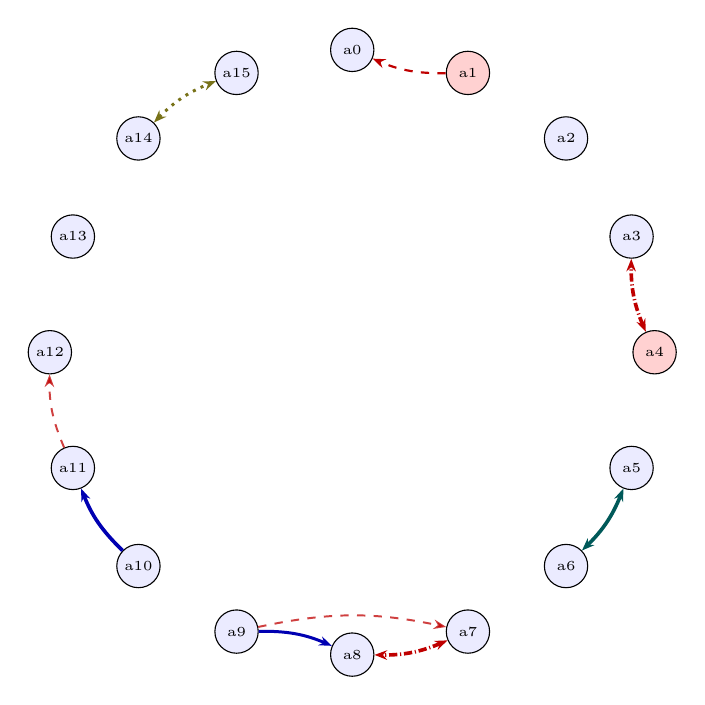
\begin{tikzpicture}[>={Stealth[length=1.6mm]}]
  \node[circle,draw,fill=blue!8,inner sep=1pt,minimum size=5.5mm,font=\tiny] (a0) at (90.0:3.84) {a0};
  \node[circle,draw,fill=red!18,inner sep=1pt,minimum size=5.5mm,font=\tiny] (a1) at (67.5:3.84) {a1};
  \node[circle,draw,fill=blue!8,inner sep=1pt,minimum size=5.5mm,font=\tiny] (a2) at (45.0:3.84) {a2};
  \node[circle,draw,fill=blue!8,inner sep=1pt,minimum size=5.5mm,font=\tiny] (a3) at (22.5:3.84) {a3};
  \node[circle,draw,fill=red!18,inner sep=1pt,minimum size=5.5mm,font=\tiny] (a4) at (0.0:3.84) {a4};
  \node[circle,draw,fill=blue!8,inner sep=1pt,minimum size=5.5mm,font=\tiny] (a5) at (-22.5:3.84) {a5};
  \node[circle,draw,fill=blue!8,inner sep=1pt,minimum size=5.5mm,font=\tiny] (a6) at (-45.0:3.84) {a6};
  \node[circle,draw,fill=blue!8,inner sep=1pt,minimum size=5.5mm,font=\tiny] (a7) at (-67.5:3.84) {a7};
  \node[circle,draw,fill=blue!8,inner sep=1pt,minimum size=5.5mm,font=\tiny] (a8) at (-90.0:3.84) {a8};
  \node[circle,draw,fill=blue!8,inner sep=1pt,minimum size=5.5mm,font=\tiny] (a9) at (-112.5:3.84) {a9};
  \node[circle,draw,fill=blue!8,inner sep=1pt,minimum size=5.5mm,font=\tiny] (a10) at (-135.0:3.84) {a10};
  \node[circle,draw,fill=blue!8,inner sep=1pt,minimum size=5.5mm,font=\tiny] (a11) at (-157.5:3.84) {a11};
  \node[circle,draw,fill=blue!8,inner sep=1pt,minimum size=5.5mm,font=\tiny] (a12) at (-180.0:3.84) {a12};
  \node[circle,draw,fill=blue!8,inner sep=1pt,minimum size=5.5mm,font=\tiny] (a13) at (-202.5:3.84) {a13};
  \node[circle,draw,fill=blue!8,inner sep=1pt,minimum size=5.5mm,font=\tiny] (a14) at (-225.0:3.84) {a14};
  \node[circle,draw,fill=blue!8,inner sep=1pt,minimum size=5.5mm,font=\tiny] (a15) at (-247.5:3.84) {a15};
  \draw[-{Stealth[length=1.6mm]}, red!75!black, dashed, line width=0.79pt] (a1) to[bend left=12] (a0);
  \draw[{Stealth[length=1.6mm]}-{Stealth[length=1.6mm]}, red!75!black, densely dashdotted, line width=1.31pt] (a4) to[bend left=12] (a3);
  \draw[{Stealth[length=1.6mm]}-{Stealth[length=1.6mm]}, teal!70!black, line width=1.31pt] (a5) to[bend left=12] (a6);
  \draw[{Stealth[length=1.6mm]}-{Stealth[length=1.6mm]}, red!75!black, densely dashdotted, line width=1.31pt] (a7) to[bend left=12] (a8);
  \draw[-{Stealth[length=1.6mm]}, blue!70!black, line width=1.08pt] (a9) to[bend left=12] (a8);
  \draw[-{Stealth[length=1.6mm]}, red!75!black, dashed, opacity=0.75, line width=0.71pt] (a9) to[bend left=12] (a7);
  \draw[-{Stealth[length=1.6mm]}, blue!70!black, line width=1.31pt] (a10) to[bend left=12] (a11);
  \draw[-{Stealth[length=1.6mm]}, red!75!black, dashed, opacity=0.75, line width=0.71pt] (a11) to[bend left=12] (a12);
  \draw[{Stealth[length=1.6mm]}-{Stealth[length=1.6mm]}, olive!80!black, dotted, line width=1.08pt] (a14) to[bend left=12] (a15);
\end{tikzpicture}
}
\\[2pt]{\footnotesize all gold edges: 9 factors}
\end{minipage}\hfill\begin{minipage}[t]{0.48\linewidth}\centering
\resizebox{!}{6.4cm}{%
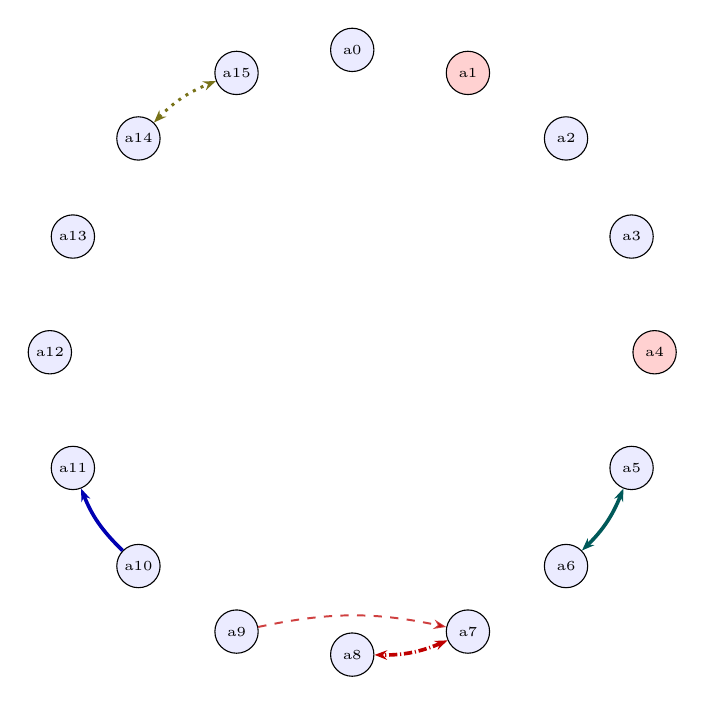
\begin{tikzpicture}[>={Stealth[length=1.6mm]}]
  \node[circle,draw,fill=blue!8,inner sep=1pt,minimum size=5.5mm,font=\tiny] (a0) at (90.0:3.84) {a0};
  \node[circle,draw,fill=red!18,inner sep=1pt,minimum size=5.5mm,font=\tiny] (a1) at (67.5:3.84) {a1};
  \node[circle,draw,fill=blue!8,inner sep=1pt,minimum size=5.5mm,font=\tiny] (a2) at (45.0:3.84) {a2};
  \node[circle,draw,fill=blue!8,inner sep=1pt,minimum size=5.5mm,font=\tiny] (a3) at (22.5:3.84) {a3};
  \node[circle,draw,fill=red!18,inner sep=1pt,minimum size=5.5mm,font=\tiny] (a4) at (0.0:3.84) {a4};
  \node[circle,draw,fill=blue!8,inner sep=1pt,minimum size=5.5mm,font=\tiny] (a5) at (-22.5:3.84) {a5};
  \node[circle,draw,fill=blue!8,inner sep=1pt,minimum size=5.5mm,font=\tiny] (a6) at (-45.0:3.84) {a6};
  \node[circle,draw,fill=blue!8,inner sep=1pt,minimum size=5.5mm,font=\tiny] (a7) at (-67.5:3.84) {a7};
  \node[circle,draw,fill=blue!8,inner sep=1pt,minimum size=5.5mm,font=\tiny] (a8) at (-90.0:3.84) {a8};
  \node[circle,draw,fill=blue!8,inner sep=1pt,minimum size=5.5mm,font=\tiny] (a9) at (-112.5:3.84) {a9};
  \node[circle,draw,fill=blue!8,inner sep=1pt,minimum size=5.5mm,font=\tiny] (a10) at (-135.0:3.84) {a10};
  \node[circle,draw,fill=blue!8,inner sep=1pt,minimum size=5.5mm,font=\tiny] (a11) at (-157.5:3.84) {a11};
  \node[circle,draw,fill=blue!8,inner sep=1pt,minimum size=5.5mm,font=\tiny] (a12) at (-180.0:3.84) {a12};
  \node[circle,draw,fill=blue!8,inner sep=1pt,minimum size=5.5mm,font=\tiny] (a13) at (-202.5:3.84) {a13};
  \node[circle,draw,fill=blue!8,inner sep=1pt,minimum size=5.5mm,font=\tiny] (a14) at (-225.0:3.84) {a14};
  \node[circle,draw,fill=blue!8,inner sep=1pt,minimum size=5.5mm,font=\tiny] (a15) at (-247.5:3.84) {a15};
  \draw[{Stealth[length=1.6mm]}-{Stealth[length=1.6mm]}, teal!70!black, line width=1.31pt] (a5) to[bend left=12] (a6);
  \draw[{Stealth[length=1.6mm]}-{Stealth[length=1.6mm]}, red!75!black, densely dashdotted, line width=1.31pt] (a7) to[bend left=12] (a8);
  \draw[-{Stealth[length=1.6mm]}, red!75!black, dashed, opacity=0.75, line width=0.71pt] (a9) to[bend left=12] (a7);
  \draw[-{Stealth[length=1.6mm]}, blue!70!black, line width=1.31pt] (a10) to[bend left=12] (a11);
  \draw[{Stealth[length=1.6mm]}-{Stealth[length=1.6mm]}, olive!80!black, dotted, line width=1.08pt] (a14) to[bend left=12] (a15);
\end{tikzpicture}
}
\\[2pt]{\footnotesize valid edges only: 5 factors}
\end{minipage}
\caption{Relation graph for \texttt{locobench-claude-5-f001-r1}. Nodes are atoms on a circle, tinted red when the item marks them non-factual (prior 0.1) and blue when factual (prior 0.9). Edges are gold relations: solid blue = entailment, dashed red = contradiction, double-headed teal = equivalence, dash-dotted red (double-headed) = exclusive (exactly-one), dotted olive (double-headed) = co-necessity (at-least-one); thickness scales with the factor probability. Ordering-only Precedence edges carry no factor and so are not drawn.}
\label{fig:graph-locobench-claude-5-f001-r1}
\end{figure}

\begin{table}[htbp]
\centering
\footnotesize
\setlength{\tabcolsep}{3.5pt}
\caption{The specific gold relations of \texttt{locobench-claude-5-f001-r1}. \textbf{$p$ used} is the factor probability the MRF received: the band midpoint, times $(1-\lambda)$ for a resolved concession, or \emph{none} for an ordering-only edge (no factor). \textbf{Valid} marks the deliberately-planted errors with their kind. \textbf{Res.} is the resolving atom of a resolved concession.}
\label{tab:rels-locobench-claude-5-f001-r1}
\begin{tabular}{lllllrll}
\toprule
ID & Endpoints & Sense & Coupling & Band & $p$ used & Valid & Res. \\
\midrule
\texttt{r000} & \texttt{a0} $\to$ \texttt{a2} & Precedence & \texttt{none} & strong & \emph{none} & \checkmark &  \\
\texttt{r001} & \texttt{a1} $\leftrightarrow$ \texttt{a0} & Contrast & \texttt{contradiction} & weak & 0.470 & $\times$ {\scriptsize false\_endpoint} &  \\
\texttt{r002} & \texttt{a4} $\leftrightarrow$ \texttt{a3} & Alternative & \texttt{exclusive} & strong & 0.925 & $\times$ {\scriptsize false\_endpoint} &  \\
\texttt{r003} & \texttt{a5} $\leftrightarrow$ \texttt{a6} & Restatement & \texttt{equivalence} & strong & 0.925 & \checkmark &  \\
\texttt{r004} & \texttt{a7} $\leftrightarrow$ \texttt{a8} & Alternative & \texttt{exclusive} & strong & 0.925 & \checkmark &  \\
\texttt{r005} & \texttt{a9} $\to$ \texttt{a8} & Instantiation & \texttt{entailment} & moderate & 0.720 & $\times$ {\scriptsize wrong\_direction} &  \\
\texttt{r006} & \texttt{a9} $\to$ \texttt{a7} & Concession & \texttt{contradiction} & moderate & 0.396 & \checkmark & \texttt{a11} \\
\texttt{r007} & \texttt{a10} $\to$ \texttt{a11} & Evidence & \texttt{entailment} & strong & 0.925 & \checkmark &  \\
\texttt{r008} & \texttt{a11} $\to$ \texttt{a12} & Concession & \texttt{contradiction} & moderate & 0.396 & $\times$ {\scriptsize wrong\_sense} & \texttt{a13} \\
\texttt{r009} & \texttt{a14} $\leftrightarrow$ \texttt{a15} & Disjunction & \texttt{co\_necessity} & moderate & 0.720 & \checkmark &  \\
\bottomrule
\end{tabular}
\end{table}

\begin{table}[htbp]
\centering
\footnotesize
\caption{Atoms of \texttt{locobench-claude-5-f001-r1}: the \texttt{factual} label, the prior it maps to, the posterior marginal $P(a_i{=}1)$ the MRF returns, and the shift. Atoms dragged below their prior are the ones the coherence structure penalises.}
\label{tab:atoms-locobench-claude-5-f001-r1}
\begin{tabular}{llrrrp{7.2cm}}
\toprule
Atom & fact & $\pi_i$ & $P(a_i{=}1)$ & $\Delta$ & Text \\
\midrule
\texttt{a0} & \checkmark & 0.90 & 0.901 & +0.001 & \footnotesize LB1 was excavated in 2003 from Liang Bua cave on the Indonesian island of Flores. \\
\texttt{a1} & $\times$ & 0.10 & 0.104 & +0.004 & \footnotesize LB1 was recovered in 2001 from the Mata Menge excavation on Flores. \\
\texttt{a2} & \checkmark & 0.90 & 0.900 & +0.000 & \footnotesize Peter Brown, Michael Morwood and colleagues described the remains as a new species, Homo floresiensis, in Nature in 2004. \\
\texttt{a3} & \checkmark & 0.90 & 0.979 & +0.079 & \footnotesize LB1's endocranial volume was measured at approximately 417 cubic centimetres. \\
\texttt{a4} & $\times$ & 0.10 & 0.021 & -0.079 & \footnotesize LB1's endocranial volume was measured at 780 cubic centimetres. \\
\texttt{a5} & \checkmark & 0.90 & 0.979 & +0.079 & \footnotesize LB1 stood about 1.06 metres tall. \\
\texttt{a6} & \checkmark & 0.90 & 0.979 & +0.079 & \footnotesize The estimated stature of LB1 was roughly three and a half feet. \\
\texttt{a7} & \checkmark & 0.90 & 0.630 & -0.270 & \footnotesize The Liang Bua remains represent a hominin species distinct from Homo sapiens. \\
\texttt{a8} & \checkmark & 0.90 & 0.767 & -0.133 & \footnotesize The Liang Bua remains are modern humans affected by a developmental pathology. \\
\texttt{a9} & \checkmark & 0.90 & 0.910 & +0.010 & \footnotesize Teuku Jacob argued that LB1 was a modern human pygmy affected by microcephaly. \\
\texttt{a10} & \checkmark & 0.90 & 0.939 & +0.039 & \footnotesize Dean Falk and colleagues built a virtual endocast of LB1 from CT scans and compared it with endocasts of microcephalic humans. \\
\texttt{a11} & \checkmark & 0.90 & 0.987 & +0.087 & \footnotesize Independent reviewers of the endocast evidence concluded that LB1's brain shape fell outside the range of microcephalic modern humans. \\
\texttt{a12} & \checkmark & 0.90 & 0.932 & +0.032 & \footnotesize Maciej Henneberg and Robert Eckhardt proposed in 2014 that LB1 was a modern human with Down syndrome. \\
\texttt{a13} & \checkmark & 0.90 & 0.900 & +0.000 & \footnotesize A comparative assessment of craniofacial and postcranial morphology determined that LB1 lacked the diagnostic features of Down syndrome. \\
\texttt{a14} & \checkmark & 0.90 & 0.929 & +0.029 & \footnotesize The Liang Bua deposits contain skeletal elements from more than one hominin individual. \\
\texttt{a15} & \checkmark & 0.90 & 0.929 & +0.029 & \footnotesize The Liang Bua deposits contain stone artefacts manufactured by hominins. \\
\bottomrule
\end{tabular}
\end{table}

\subsection{Archaeology -- base (\texttt{locobench-claude-5-f002-r1})}

\textbf{Topic:} Archaeology (Humanities). \textbf{Family:} \texttt{f002} (CONFLICT), rung 1 (\emph{base}). \textbf{Scores:} mean-marg $= 0.792$, consist $= 0.304$, reified $= 0.330$, log-Z $= 0.367$.



\paragraph{Framing question.} \emph{How do archaeologists adjudicate between rival interpretations when a site's stratigraphy and its radiocarbon dates appear to disagree about when a settlement was abandoned?}



\paragraph{Response.} {\small When a settlement's stratigraphic sequence and its radiocarbon determinations point to different abandonment dates, the dispute is settled not by privileging one class of evidence but by specifying precisely what each of them measures. Radiocarbon dating measures the residual carbon-14 activity of organic samples. The same technique, by contrast, measures the decay of potassium-40 within bone apatite. Stratigraphy delivers something of a quite different order: an ordinal record of deposition, which constrains sequence without ever yielding a calendar year on its own.

A further complication sits between the laboratory result and any statement about the past. Raw radiocarbon ages must be calibrated against a tree-ring-based curve to yield calendar dates; specifically, IntCal20 is the agreed calibration curve for Northern Hemisphere terrestrial samples. Until that conversion is performed, a determination cannot be compared with a stratigraphic expectation at all, and a good deal of apparent conflict dissolves once the irregular calibrated interval replaces the single mean age.

Excavators record the relative order of deposits in a Harris matrix, and only after that ordering has been established does Bayesian chronological modelling combine stratigraphic ordering as a prior with the radiocarbon determinations as likelihoods. OxCal, software used to construct Bayesian age models for archaeological sequences, is what brings about that union of prior and likelihood, and the resulting formalism converts an impressionistic clash of evidence into a set of testable propositions about which samples belong where.

Reconciliation then usually turns on taphonomy. Residual charcoal redeposited from earlier deposits yields ages older than the layer containing it, whereas the old wood effect makes a dated sample appear younger than the event it is meant to date. Both processes bear on the disputed horizon at the site in question, where the excavated material was reassessed sample by sample and context by context. The charcoal in the abandonment layer was residual material derived from earlier occupation deposits, which is evidence for the general principle that redeposited charcoal reads older than its enclosing deposit; and at least one of that residual origin or a disturbance of the abandonment layer by pit digging during a later phase of activity must hold, perhaps both.

Although all twelve radiocarbon determinations from the abandonment horizon were statistically consistent with one another, the residual origin of the charcoal remained the more economical reading of the sequence, since close agreement among samples drawn from a single reworked population is exactly what redeposition predicts. Either that mutual consistency holds, or at least one of the twelve was a statistical outlier; the two cannot both be true, and one of them must. Judgements of this kind are not left to the excavator alone but are submitted to external scrutiny before publication. The peer-review panel concluded that the charcoal dates were residual rather than contemporary with the abandonment deposit, and that verdict settles the apparent tension: a set of internally consistent determinations that are collectively too old is no obstacle to a later abandonment, because their agreement reflects a common source rather than a common event. Chronological resolution in such cases is properly reported as a probability interval rather than a point estimate. The Bayesian model placed the settlement's abandonment between 1130 and 1090 BCE at 95\% probability — in other words, the model's 95\% probability estimate for abandonment of the settlement spanned the four decades from 1130 to 1090 BCE. Adjudication, on this account, is neither a vote between stratigraphers and physicists nor an appeal to authority, but the explicit modelling of sample provenance, calibration, and depositional order within a single framework whose assumptions can be inspected, criticized, and revised as new determinations accumulate.}

\begin{figure}[htbp]
\centering
\begin{minipage}[t]{0.48\linewidth}\centering
\resizebox{!}{6.4cm}{%
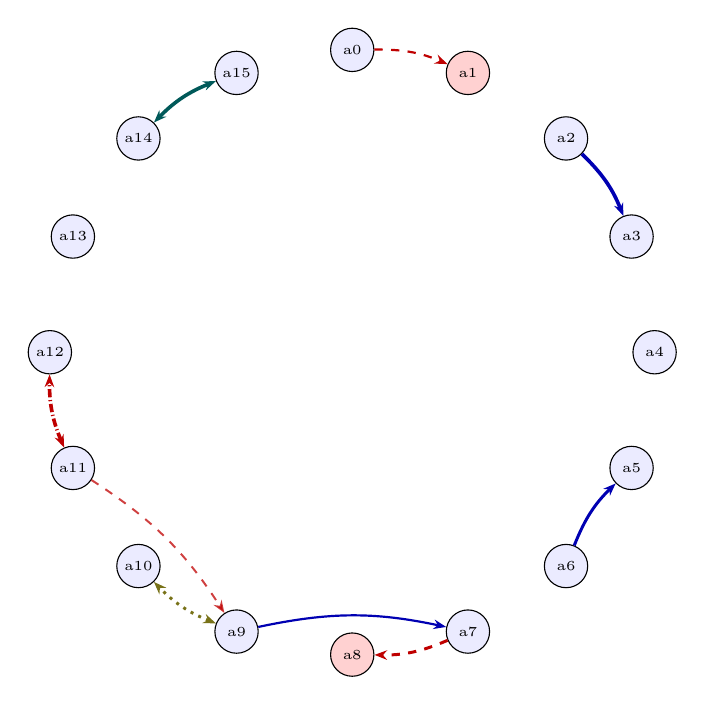
\begin{tikzpicture}[>={Stealth[length=1.6mm]}]
  \node[circle,draw,fill=blue!8,inner sep=1pt,minimum size=5.5mm,font=\tiny] (a0) at (90.0:3.84) {a0};
  \node[circle,draw,fill=red!18,inner sep=1pt,minimum size=5.5mm,font=\tiny] (a1) at (67.5:3.84) {a1};
  \node[circle,draw,fill=blue!8,inner sep=1pt,minimum size=5.5mm,font=\tiny] (a2) at (45.0:3.84) {a2};
  \node[circle,draw,fill=blue!8,inner sep=1pt,minimum size=5.5mm,font=\tiny] (a3) at (22.5:3.84) {a3};
  \node[circle,draw,fill=blue!8,inner sep=1pt,minimum size=5.5mm,font=\tiny] (a4) at (0.0:3.84) {a4};
  \node[circle,draw,fill=blue!8,inner sep=1pt,minimum size=5.5mm,font=\tiny] (a5) at (-22.5:3.84) {a5};
  \node[circle,draw,fill=blue!8,inner sep=1pt,minimum size=5.5mm,font=\tiny] (a6) at (-45.0:3.84) {a6};
  \node[circle,draw,fill=blue!8,inner sep=1pt,minimum size=5.5mm,font=\tiny] (a7) at (-67.5:3.84) {a7};
  \node[circle,draw,fill=red!18,inner sep=1pt,minimum size=5.5mm,font=\tiny] (a8) at (-90.0:3.84) {a8};
  \node[circle,draw,fill=blue!8,inner sep=1pt,minimum size=5.5mm,font=\tiny] (a9) at (-112.5:3.84) {a9};
  \node[circle,draw,fill=blue!8,inner sep=1pt,minimum size=5.5mm,font=\tiny] (a10) at (-135.0:3.84) {a10};
  \node[circle,draw,fill=blue!8,inner sep=1pt,minimum size=5.5mm,font=\tiny] (a11) at (-157.5:3.84) {a11};
  \node[circle,draw,fill=blue!8,inner sep=1pt,minimum size=5.5mm,font=\tiny] (a12) at (-180.0:3.84) {a12};
  \node[circle,draw,fill=blue!8,inner sep=1pt,minimum size=5.5mm,font=\tiny] (a13) at (-202.5:3.84) {a13};
  \node[circle,draw,fill=blue!8,inner sep=1pt,minimum size=5.5mm,font=\tiny] (a14) at (-225.0:3.84) {a14};
  \node[circle,draw,fill=blue!8,inner sep=1pt,minimum size=5.5mm,font=\tiny] (a15) at (-247.5:3.84) {a15};
  \draw[-{Stealth[length=1.6mm]}, red!75!black, dashed, line width=0.79pt] (a0) to[bend left=12] (a1);
  \draw[-{Stealth[length=1.6mm]}, blue!70!black, line width=1.31pt] (a2) to[bend left=12] (a3);
  \draw[-{Stealth[length=1.6mm]}, blue!70!black, line width=1.08pt] (a6) to[bend left=12] (a5);
  \draw[-{Stealth[length=1.6mm]}, red!75!black, dashed, line width=1.08pt] (a7) to[bend left=12] (a8);
  \draw[-{Stealth[length=1.6mm]}, blue!70!black, line width=0.79pt] (a9) to[bend left=12] (a7);
  \draw[{Stealth[length=1.6mm]}-{Stealth[length=1.6mm]}, olive!80!black, dotted, line width=1.08pt] (a9) to[bend left=12] (a10);
  \draw[-{Stealth[length=1.6mm]}, red!75!black, dashed, opacity=0.75, line width=0.71pt] (a11) to[bend left=12] (a9);
  \draw[{Stealth[length=1.6mm]}-{Stealth[length=1.6mm]}, red!75!black, densely dashdotted, line width=1.31pt] (a11) to[bend left=12] (a12);
  \draw[{Stealth[length=1.6mm]}-{Stealth[length=1.6mm]}, teal!70!black, line width=1.31pt] (a14) to[bend left=12] (a15);
\end{tikzpicture}
}
\\[2pt]{\footnotesize all gold edges: 9 factors}
\end{minipage}\hfill\begin{minipage}[t]{0.48\linewidth}\centering
\resizebox{!}{6.4cm}{%
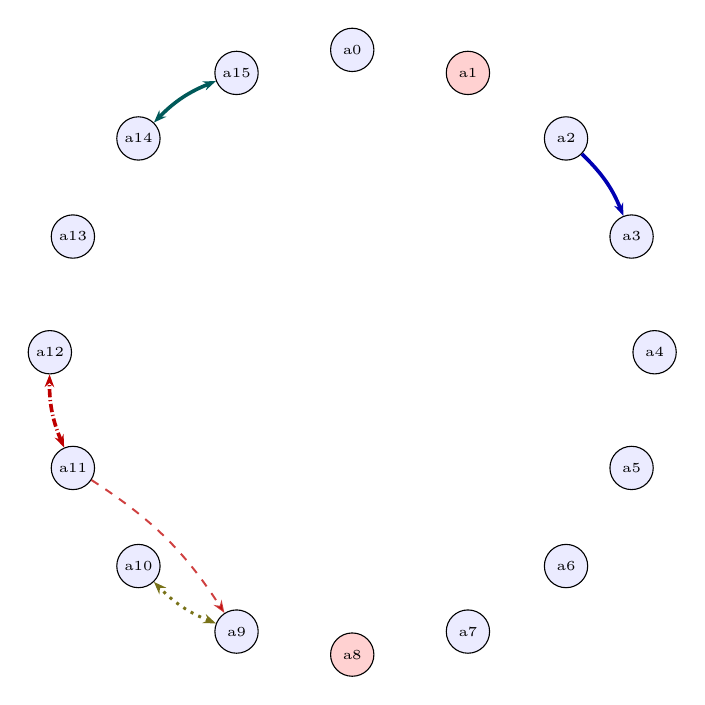
\begin{tikzpicture}[>={Stealth[length=1.6mm]}]
  \node[circle,draw,fill=blue!8,inner sep=1pt,minimum size=5.5mm,font=\tiny] (a0) at (90.0:3.84) {a0};
  \node[circle,draw,fill=red!18,inner sep=1pt,minimum size=5.5mm,font=\tiny] (a1) at (67.5:3.84) {a1};
  \node[circle,draw,fill=blue!8,inner sep=1pt,minimum size=5.5mm,font=\tiny] (a2) at (45.0:3.84) {a2};
  \node[circle,draw,fill=blue!8,inner sep=1pt,minimum size=5.5mm,font=\tiny] (a3) at (22.5:3.84) {a3};
  \node[circle,draw,fill=blue!8,inner sep=1pt,minimum size=5.5mm,font=\tiny] (a4) at (0.0:3.84) {a4};
  \node[circle,draw,fill=blue!8,inner sep=1pt,minimum size=5.5mm,font=\tiny] (a5) at (-22.5:3.84) {a5};
  \node[circle,draw,fill=blue!8,inner sep=1pt,minimum size=5.5mm,font=\tiny] (a6) at (-45.0:3.84) {a6};
  \node[circle,draw,fill=blue!8,inner sep=1pt,minimum size=5.5mm,font=\tiny] (a7) at (-67.5:3.84) {a7};
  \node[circle,draw,fill=red!18,inner sep=1pt,minimum size=5.5mm,font=\tiny] (a8) at (-90.0:3.84) {a8};
  \node[circle,draw,fill=blue!8,inner sep=1pt,minimum size=5.5mm,font=\tiny] (a9) at (-112.5:3.84) {a9};
  \node[circle,draw,fill=blue!8,inner sep=1pt,minimum size=5.5mm,font=\tiny] (a10) at (-135.0:3.84) {a10};
  \node[circle,draw,fill=blue!8,inner sep=1pt,minimum size=5.5mm,font=\tiny] (a11) at (-157.5:3.84) {a11};
  \node[circle,draw,fill=blue!8,inner sep=1pt,minimum size=5.5mm,font=\tiny] (a12) at (-180.0:3.84) {a12};
  \node[circle,draw,fill=blue!8,inner sep=1pt,minimum size=5.5mm,font=\tiny] (a13) at (-202.5:3.84) {a13};
  \node[circle,draw,fill=blue!8,inner sep=1pt,minimum size=5.5mm,font=\tiny] (a14) at (-225.0:3.84) {a14};
  \node[circle,draw,fill=blue!8,inner sep=1pt,minimum size=5.5mm,font=\tiny] (a15) at (-247.5:3.84) {a15};
  \draw[-{Stealth[length=1.6mm]}, blue!70!black, line width=1.31pt] (a2) to[bend left=12] (a3);
  \draw[{Stealth[length=1.6mm]}-{Stealth[length=1.6mm]}, olive!80!black, dotted, line width=1.08pt] (a9) to[bend left=12] (a10);
  \draw[-{Stealth[length=1.6mm]}, red!75!black, dashed, opacity=0.75, line width=0.71pt] (a11) to[bend left=12] (a9);
  \draw[{Stealth[length=1.6mm]}-{Stealth[length=1.6mm]}, red!75!black, densely dashdotted, line width=1.31pt] (a11) to[bend left=12] (a12);
  \draw[{Stealth[length=1.6mm]}-{Stealth[length=1.6mm]}, teal!70!black, line width=1.31pt] (a14) to[bend left=12] (a15);
\end{tikzpicture}
}
\\[2pt]{\footnotesize valid edges only: 5 factors}
\end{minipage}
\caption{Relation graph for \texttt{locobench-claude-5-f002-r1}. Nodes are atoms on a circle, tinted red when the item marks them non-factual (prior 0.1) and blue when factual (prior 0.9). Edges are gold relations: solid blue = entailment, dashed red = contradiction, double-headed teal = equivalence, dash-dotted red (double-headed) = exclusive (exactly-one), dotted olive (double-headed) = co-necessity (at-least-one); thickness scales with the factor probability. Ordering-only Precedence edges carry no factor and so are not drawn.}
\label{fig:graph-locobench-claude-5-f002-r1}
\end{figure}

\begin{table}[htbp]
\centering
\footnotesize
\setlength{\tabcolsep}{3.5pt}
\caption{The specific gold relations of \texttt{locobench-claude-5-f002-r1}. \textbf{$p$ used} is the factor probability the MRF received: the band midpoint, times $(1-\lambda)$ for a resolved concession, or \emph{none} for an ordering-only edge (no factor). \textbf{Valid} marks the deliberately-planted errors with their kind. \textbf{Res.} is the resolving atom of a resolved concession.}
\label{tab:rels-locobench-claude-5-f002-r1}
\begin{tabular}{lllllrll}
\toprule
ID & Endpoints & Sense & Coupling & Band & $p$ used & Valid & Res. \\
\midrule
\texttt{r000} & \texttt{a0} $\leftrightarrow$ \texttt{a1} & Contrast & \texttt{contradiction} & weak & 0.470 & $\times$ {\scriptsize false\_endpoint} &  \\
\texttt{r001} & \texttt{a2} $\to$ \texttt{a3} & Instantiation & \texttt{entailment} & strong & 0.925 & \checkmark &  \\
\texttt{r002} & \texttt{a4} $\to$ \texttt{a5} & Precedence & \texttt{none} & moderate & \emph{none} & \checkmark &  \\
\texttt{r003} & \texttt{a6} $\to$ \texttt{a5} & Cause-Effect & \texttt{entailment} & moderate & 0.720 & $\times$ {\scriptsize wrong\_sense} &  \\
\texttt{r004} & \texttt{a7} $\leftrightarrow$ \texttt{a8} & Contrast & \texttt{contradiction} & moderate & 0.720 & $\times$ {\scriptsize false\_endpoint} &  \\
\texttt{r005} & \texttt{a9} $\to$ \texttt{a7} & Evidence & \texttt{entailment} & weak & 0.470 & $\times$ {\scriptsize wrong\_direction} &  \\
\texttt{r006} & \texttt{a9} $\leftrightarrow$ \texttt{a10} & Disjunction & \texttt{co\_necessity} & moderate & 0.720 & \checkmark &  \\
\texttt{r007} & \texttt{a11} $\to$ \texttt{a9} & Concession & \texttt{contradiction} & moderate & 0.396 & \checkmark & \texttt{a13} \\
\texttt{r008} & \texttt{a11} $\leftrightarrow$ \texttt{a12} & Alternative & \texttt{exclusive} & strong & 0.925 & \checkmark &  \\
\texttt{r009} & \texttt{a14} $\leftrightarrow$ \texttt{a15} & Restatement & \texttt{equivalence} & strong & 0.925 & \checkmark &  \\
\bottomrule
\end{tabular}
\end{table}

\begin{table}[htbp]
\centering
\footnotesize
\caption{Atoms of \texttt{locobench-claude-5-f002-r1}: the \texttt{factual} label, the prior it maps to, the posterior marginal $P(a_i{=}1)$ the MRF returns, and the shift. Atoms dragged below their prior are the ones the coherence structure penalises.}
\label{tab:atoms-locobench-claude-5-f002-r1}
\begin{tabular}{llrrrp{7.2cm}}
\toprule
Atom & fact & $\pi_i$ & $P(a_i{=}1)$ & $\Delta$ & Text \\
\midrule
\texttt{a0} & \checkmark & 0.90 & 0.895 & -0.005 & \footnotesize Radiocarbon dating measures the residual carbon-14 activity of organic samples. \\
\texttt{a1} & $\times$ & 0.10 & 0.110 & +0.010 & \footnotesize Radiocarbon dating measures the decay of potassium-40 within bone apatite. \\
\texttt{a2} & \checkmark & 0.90 & 0.938 & +0.038 & \footnotesize Raw radiocarbon ages must be calibrated against a tree-ring-based curve to yield calendar dates. \\
\texttt{a3} & \checkmark & 0.90 & 0.985 & +0.085 & \footnotesize IntCal20 is the agreed calibration curve for Northern Hemisphere terrestrial samples. \\
\texttt{a4} & \checkmark & 0.90 & 0.900 & +0.000 & \footnotesize Excavators record the relative order of deposits in a Harris matrix. \\
\texttt{a5} & \checkmark & 0.90 & 0.954 & +0.054 & \footnotesize Bayesian chronological modelling combines stratigraphic ordering as a prior with the radiocarbon determinations as likelihoods. \\
\texttt{a6} & \checkmark & 0.90 & 0.924 & +0.024 & \footnotesize OxCal is software used to construct Bayesian age models for archaeological sequences. \\
\texttt{a7} & \checkmark & 0.90 & 0.916 & +0.016 & \footnotesize Residual charcoal redeposited from earlier deposits yields ages older than the layer containing it. \\
\texttt{a8} & $\times$ & 0.10 & 0.046 & -0.054 & \footnotesize The old wood effect makes a dated sample appear younger than the event it is meant to date. \\
\texttt{a9} & \checkmark & 0.90 & 0.942 & +0.042 & \footnotesize The charcoal in the abandonment layer was residual material derived from earlier occupation deposits. \\
\texttt{a10} & \checkmark & 0.90 & 0.929 & +0.029 & \footnotesize The abandonment layer was disturbed by pit digging during a later phase of activity. \\
\texttt{a11} & \checkmark & 0.90 & 0.669 & -0.231 & \footnotesize All twelve radiocarbon determinations from the abandonment horizon were statistically consistent with one another. \\
\texttt{a12} & \checkmark & 0.90 & 0.610 & -0.290 & \footnotesize At least one of the twelve determinations from the abandonment horizon was a statistical outlier. \\
\texttt{a13} & \checkmark & 0.90 & 0.900 & +0.000 & \footnotesize The peer-review panel concluded that the charcoal dates were residual rather than contemporary with the abandonment deposit. \\
\texttt{a14} & \checkmark & 0.90 & 0.979 & +0.079 & \footnotesize The Bayesian model placed the settlement's abandonment between 1130 and 1090 BCE at 95\% probability. \\
\texttt{a15} & \checkmark & 0.90 & 0.979 & +0.079 & \footnotesize The model's 95\% probability estimate for abandonment of the settlement spanned the four decades from 1130 to 1090 BCE. \\
\bottomrule
\end{tabular}
\end{table}

\section{Findings}

\begin{itemize}
\item \textbf{The corpus's gold relations are constant within a family, so the ladder is untestable from gold alone.} 2 of 2 families carry identical gold relations across all five rungs while their response texts differ. Every readout is flat within a family, and the strict-increase constraints fail by construction. This is a defect in the generated corpus, not a property of the LCS pipeline. It is now fixed in the generator (see Section~\ref{sec:ladder}); applying the corrected per-rung transforms to these base rungs makes $\log Z$ strictly monotone up both ladders. The tables here describe the dataset as generated, before that fix.
\item \textbf{The readouts differ sharply in sensitivity.} Across the 10 scored items \texttt{mean\_marginal} spans only $[0.792, 0.799]$, while \texttt{consistency} spans $[0.029, 0.304]$. With atom priors pinned at $0.9/0.1$ the mean marginal is dominated by those priors and moves little; the conflict-sensitive readouts are what register the contradiction structure. For a benchmark whose families vary conflict structure, \texttt{consistency} and \texttt{log\_partition} are the discriminating readouts.
\item \textbf{The planted invalid relations carry most of the incoherence.} Dropping them changes \texttt{consistency} by 0.046 to 0.291 across items. The planted errors are largely conflict edges anchored to a false endpoint, so they add active contradictions, and the intended-correct subgraph is markedly more coherent. That the effect runs in this direction is a sanity check that the gold labels and the MRF encoding agree about which edges are the damaging ones.
\item \textbf{Relation counts and factor counts are not the same number.} Of 100 gold relations, 10 are Precedence edges that couple no truth values and never reach the MRF, and 40 are deliberately invalid. Any comparison of graph density needs both figures; Table~\ref{tab:dataset} reports them separately for that reason.
\end{itemize}

\section{Threats to validity}

\begin{itemize}
\item \textbf{Gold relations are labels, not measurements.} The factor probability is a band midpoint, so a \texttt{strong} edge enters at exactly 0.925 whatever the underlying text supports. Nothing here tests the miner's calibration: this evaluates the MRF encoding and the readouts \emph{given} perfect relation labels. Treat these scores as a reference point for a mined arm, not as a mining result.
\item \textbf{Two families is a small sample.} The dataset has 2 families over 10 items, all generated by one model. The spreads quoted above describe this dataset; no significance claim is made or implied.
\item \textbf{The ladder result is a corpus measurement.} Because gold relations repeat across rungs, the pass rates in the ordering-constraint tables report a property of the generated data. They are not evidence about whether the LCS pipeline ranks coherence correctly --- that question needs per-rung relations.
\item \textbf{The concession discount is applied from the label.} Using the item's \texttt{resolver\_atom\_id} bypasses the text heuristic a live miner must use, so the resolved-concession behaviour shown here is the best case for that mechanism.
\item \textbf{Inference is approximate in general.} Merlin runs weighted mini-bucket at a finite $i$-bound. On these 16-atom networks the induced width is small enough that it reports exact inference, but the normalized log-partition also depends on a MAP floor and a contradiction-free ceiling, so it is the readout most sensitive to any approximation.
\end{itemize}

\end{document}
